\chapter{Example Chapter}
\label{chap:example}

This chapter is a cheat sheet. Keep it open while you write, then delete it.

\section{Figures}

Put image files in the \texttt{images/} folder and include them by name,
without the extension: \verb|\includegraphics[width=0.6\linewidth]{my-figure}|.
\Cref{fig:pipeline} is drawn directly in \LaTeX{} with TikZ.

\begin{figure}[H]
  \centering
  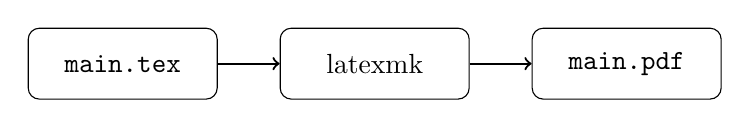
\begin{tikzpicture}[node distance=3.2cm, every node/.style={draw, rounded corners, minimum width=2.4cm, minimum height=0.9cm, align=center}]
    \node (tex) {\texttt{main.tex}};
    \node (latexmk) [right of=tex] {latexmk};
    \node (pdf) [right of=latexmk] {\texttt{main.pdf}};
    \draw[->, thick] (tex) -- (latexmk);
    \draw[->, thick] (latexmk) -- (pdf);
  \end{tikzpicture}
  \caption{What happens when you press save.}
  \label{fig:pipeline}
\end{figure}

\section{Tables}

\Cref{tab:toolchain} uses \texttt{booktabs} rules, which look cleaner than
vertical lines.

\begin{table}[H]
  \centering
  \begin{tabularx}{\linewidth}{l X l}
    \toprule
    \textbf{Tool} & \textbf{Role} & \textbf{Needed by} \\
    \midrule
    \TeX{} distribution & Compilers and packages (MiKTeX or \TeX{} Live) & everything \\
    Perl & Runs \texttt{latexmk} & automatic builds \\
    Pygments & Syntax highlighting & \texttt{minted} \\
    Biber & Bibliography processing & \texttt{biblatex} \\
    \bottomrule
  \end{tabularx}
  \caption{The toolchain behind this template.}
  \label{tab:toolchain}
\end{table}

\section{Code}

Code blocks are highlighted by \texttt{minted}, as in \cref{lst:hello}.
Short inline code works too: \mintinline{python}{print("hi")}.

\begin{listing}[H]
  \begin{minted}{python}
def greet(name: str) -> str:
    """Return a greeting."""
    return f"Hello, {name}!"

print(greet("LaTeX"))
  \end{minted}
  \caption{A Python function.}
  \label{lst:hello}
\end{listing}

\section{Equations}

Numbered equations can be referenced like any other element, see
\cref{eq:mean}:
\begin{equation}
  \bar{x} = \frac{1}{n} \sum_{i=1}^{n} x_i
  \label{eq:mean}
\end{equation}

\section{Citations and acronyms}

Cite entries from \texttt{references.bib} with \verb|\cite{key}|, for example
the \TeX{}book \cite{knuth1984texbook} or the VS Code extension used here
\cite{latexworkshop}. Acronyms are declared in \texttt{acronyms.tex}: the
first use of \verb|\ac{API}| prints ``\ac{API}'', the next ones print
``\ac{API}''.

\section{Lists}

\begin{itemize}
  \item A bullet point.
  \item Another one, with \textbf{bold} and \emph{emphasis}.
\end{itemize}

\begin{enumerate}
  \item A numbered step.
  \item The next step.
\end{enumerate}
